\documentclass{beamer} % [mathserif]
\usepackage{amsmath}
\usepackage{graphicx}
\usepackage{subfigure}
\usepackage{wrapfig}
\usepackage{booktabs}
\usepackage{hyperref}
\usepackage{media9}
% \usepackage{pgfplots}
% \pgfplotsset{compat=1.18}
% \usepgfplotslibrary{dateplot}
% \usepackage{tipa}
% \usepackage{epstopdf} % this is needed for windows Texworks
\usepackage[absolute,overlay]{textpos} % ,showboxes

\setlength{\TPHorizModule}{1in}
\TPVertModule=\TPHorizModule

\DeclareGraphicsExtensions{.eps}

\usetheme{Marburg}
% \usetheme{Berkeley}
% \usecolortheme{rose}
\definecolor{naublue}{HTML}{002454}
\definecolor{nauyellow}{HTML}{FAC01A}
%\setbeamercolor{structure}{bg=nauyellow, fg=naublue}
\setbeamercolor{palette primary}{bg=nauyellow, fg=naublue}
\setbeamercolor{palette secondary}{bg=nauyellow, fg=naublue}
%%%% See https://en.wikibooks.org/wiki/LaTeX/Presentations#User-defined_themes
% \setbeamercolor{alerted text}{fg=orange}
% \setbeamercolor{background canvas}{bg=white}
% \setbeamercolor{block body alerted}{bg=normal text.bg!90!black}
% \setbeamercolor{block body}{bg=normal text.bg!90!black}
% \setbeamercolor{block body example}{bg=normal text.bg!90!black}
% \setbeamercolor{block title alerted}{use={normal text,alerted text},fg=alerted text.fg!75!normal text.fg,bg=normal text.bg!75!black}
% \setbeamercolor{block title}{bg=blue}
% \setbeamercolor{block title example}{use={normal text,example text},fg=example text.fg!75!normal text.fg,bg=normal text.bg!75!black}
% \setbeamercolor{fine separation line}{}
\setbeamercolor{frametitle}{fg=naublue}
% \setbeamercolor{item projected}{fg=black}
% \setbeamercolor{normal text}{bg=black,fg=yellow}
% \setbeamercolor{palette sidebar primary}{use=normal text,fg=normal text.fg}
\setbeamercolor{palette sidebar primary}{bg=naublue, fg=nauyellow}
% \setbeamercolor{palette sidebar quaternary}{use=structure,fg=structure.fg}
% \setbeamercolor{palette sidebar secondary}{use=structure,fg=structure.fg}
% \setbeamercolor{palette sidebar tertiary}{use=normal text,fg=normal text.fg}
\setbeamercolor{section in sidebar}{fg=nauyellow, bg=naublue}
\setbeamercolor{section in sidebar shaded}{fg=white}
% \setbeamercolor{separation line}{}
% \setbeamercolor{sidebar}{bg=red}
% \setbeamercolor{sidebar}{parent=palette primary}
% \setbeamercolor{structure}{bg=black, fg=green}
% \setbeamercolor{subsection in sidebar}{fg=brown}
% \setbeamercolor{subsection in sidebar shaded}{fg=grey}
\setbeamercolor{title}{fg=naublue}
% \setbeamercolor{titlelike}{fg=brown}

% \usepackage[latin1]{inputenc}

%%%% See https://en.wikibooks.org/wiki/LaTeX/Presentations#Title_page_and_author_information
\title[INF632 (EE499/EE599)]{Wearable Technologies and Applications\\(Wearable Informatics)} %
\author{Winfree}
\date{Lecture 2}
%\institute{Northern Arizona University}

%\logo{\includegraphics[width=.5in]{figures/logo}}
% \setbeameroption{show notes on second screen}

\begin{document}
	\maketitle


% \section[Outline]{}
% \frame{\tableofcontents}

% \begin{frame}
%   \frametitle{Image Example}
%   \includegraphics[width=0.8\linewidth]{figures/_seikowrist.jpg}
% \end{frame}

\section{Dimensions of Functionality}
	\subsection{Axes}
	\begin{frame}
		\frametitle{Axes as a Framework}
		\begin{columns}
			\begin{column}{.65\linewidth}
				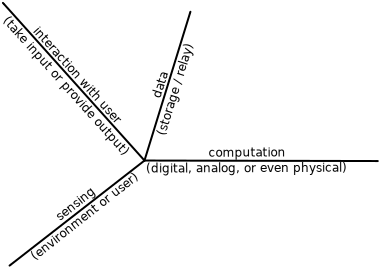
\includegraphics[width=1\linewidth]{figures/4axes.png}
			\end{column}
			\begin{column}{.35\linewidth}
				\begin{itemize}
					\item Four dimensions of functionality.
					\item Each axis is not necessarily orthogonal to any other.
				\end{itemize}
			\end{column}
		\end{columns}
	\end{frame}
	\begin{frame}
		\frametitle{Sensing}
		\begin{columns}
			\begin{column}{.65\linewidth}
				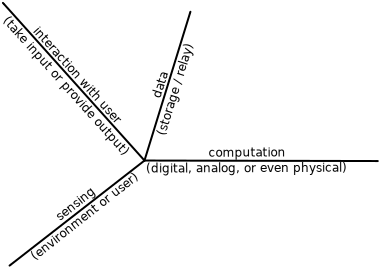
\includegraphics[width=1\linewidth]{figures/4axes.png}
			\end{column}
			\begin{column}{.35\linewidth}
				\begin{itemize}
					\item Environmental
					\begin{itemize}
						\item Temperature (not skin)
						\item Location
						\item Air quality
					\end{itemize}
					\item Wearer (user)
					\begin{itemize}
						\item Temperature (e.g. skin)
						\item Heart Rate
						\item Physical Activity Level
					\end{itemize}
				\end{itemize}
			\end{column}
		\end{columns}
	\end{frame}
	\begin{frame}
		\frametitle{Data}
		\begin{columns}
			\begin{column}{.65\linewidth}
				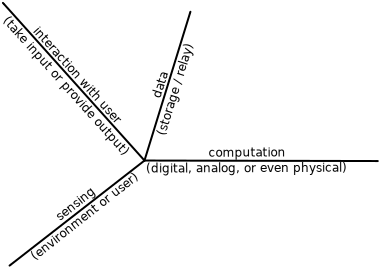
\includegraphics[width=1\linewidth]{figures/4axes.png}
			\end{column}
			\begin{column}{.35\linewidth}
				\begin{itemize}
					\item Storage
					\begin{itemize}
						\item Local
						\item No storage - process and throw away
					\end{itemize}
					\item Relay
					\begin{itemize}
						\item Physical storage - SD card
						\item Wired on command
						\item Wireless
						\item Continuous or Staged
					\end{itemize}
				\end{itemize}
			\end{column}
		\end{columns}
	\end{frame}
	\begin{frame}
		\frametitle{Interaction with the Wearer (Human Comp. Interaction - HCI)}
		\begin{columns}
			\begin{column}{.65\linewidth}
				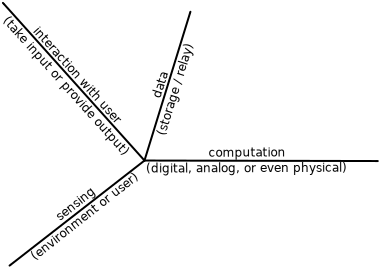
\includegraphics[width=1\linewidth]{figures/4axes.png}
			\end{column}
			\begin{column}{.35\linewidth}
				\begin{itemize}
					\item Input
					\begin{itemize}
						\item Direct entry
						\item Motion
						\item Voice Command
					\end{itemize}
					\item Output
					\begin{itemize}
						\item Audio
						\item Haptic
						\item Visual
					\end{itemize}
				\end{itemize}
			\end{column}
		\end{columns}
	\end{frame}
	\begin{frame}
		\frametitle{Computation}
		\begin{columns}
			\begin{column}{.65\linewidth}
				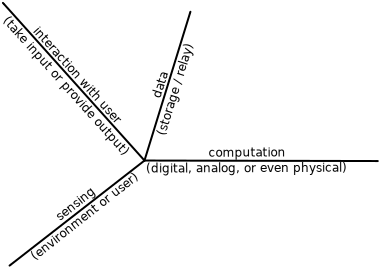
\includegraphics[width=1\linewidth]{figures/4axes.png}
			\end{column}
			\begin{column}{.35\linewidth}
				\begin{itemize}
					\item Mechanical
					\item Analog
					\item Digital
				\end{itemize}
			\end{column}
		\end{columns}
	\end{frame}
	
\section{Early Examples}
	\subsection{Rivet Glasses}
	\begin{frame}
		\frametitle{Rivet Glasses}
		\begin{columns}
			\begin{column}{.70\linewidth}
				\begin{itemize}
					\item First clear exemplar of wearable technology.
					\item Corrective glasses (with a convex lens) - 13th century in Italy. Two lenses held together by a rivet; no arms to rest on the ears.
					\item Function - Modify information (images) through a mechanical process (the lens) for the wearer (user) - mechanical computing.\footnote{https://en.wikipedia.org/wiki/Glasses, https://www.medievalchronicles.com/medieval-history/medieval-inventions-list/eyeglasses/}
				\end{itemize}
			\end{column}
			\begin{column}{.30\linewidth}
				\includegraphics[width=1\linewidth]{figures/Conrad-von-Soest-Brillenapostel-1403.jpg}
			\end{column}
		\end{columns}
	\end{frame}
	
	\subsection{Countess of Lovelace}
	\begin{frame}
		\frametitle{Countess of Lovelace}
		\begin{columns}
			\begin{column}{.70\linewidth}
				``Augusta Ada King-Noel, Countess of Lovelace (Ada Lovelace) was an English mathematician and writer, chiefly known for her work on Charles Babbage's early mechanical general-purpose computer, the Analytical Engine. Her notes on the engine include what is recognized as the first algorithm intended to be carried out by a machine. As a result, she is often regarded as the first computer programmer.'' \footnote{\url{https://en.wikipedia.org/wiki/Ada_Lovelace}}
			\end{column}
			\begin{column}{.30\linewidth}
				\includegraphics[width=1\linewidth]{figures/Ada_Lovelace_portrait.jpg}
			\end{column}
		\end{columns}
	\end{frame}
	\subsection{Roulette}
	\begin{frame}
		\frametitle{Roulette Computer}
		\begin{columns}
			\begin{column}{.70\linewidth}
				August of 1961 Edward O. Thorp and Claude Shannon, of MIT
				
				``They worked as a team. Shannon watched the wheel, clandestinely clocking the speeds of the rotor and the ball by flipping micro switches in his shoe with his big toe. The signals coursed through wires that ran up his pant leg to a small computer strapped to his waist. The machine calculated the ball's final resting position and then transmitted this prediction wirelessly to a receiver under Thorp's shirt. Through a tiny speaker in his ear, Thorp heard one of eight distinct tones that advised him on how to bet.''\footnote{\url{http://spectrum.ieee.org/consumer-electronics/portable-devices/wearable-computers-will- transform-language}}
			\end{column}
			\begin{column}{.30\linewidth}
				\includegraphics[width=1\linewidth]{figures/thorp3-viafriend620-1379361753.jpg}
			\end{column}
		\end{columns}
	\end{frame}
	
\section{``Recent'' Examples}
	\subsection{Computing on the Wrist}
	\begin{frame}
		\frametitle{Computing on the Wrist}
		\begin{columns}
			\begin{column}{.30\linewidth}
				Casio CA-90 (1970s)
				
				\includegraphics[width=1\linewidth]{figures/Casio-CA90.jpg}
			\end{column}
			\begin{column}{.40\linewidth}
% 				\begin{itemize}
% 					\item Casio CA-90 (1970s)
% 					\item Seiko UC-2100 (1984?)
% 					\item Casio Data Bank (1980s to current!)
% 				\end{itemize}
				Seiko UC-2100 (1984?)
				
				\includegraphics[width=1\linewidth]{figures/_seikowrist.jpg}
			\end{column}
			\begin{column}{.30\linewidth}
				Casio Data Bank (1980s to current!)
				
				\includegraphics[width=1\linewidth]{figures/Calculatorwatch.jpg}
			\end{column}
		\end{columns}
	\end{frame}
	\subsection{Environmental Sensing}
	\begin{frame}
		\frametitle{Environmental Sensing}
		\begin{columns}
			\begin{column}{.33\linewidth}
				\includegraphics[width=1\linewidth]{figures/airbot.jpg}
			\end{column}
			\begin{column}{.33\linewidth}
				\includegraphics[width=1\linewidth]{figures/sensaris-air-sensor.jpg}
			\end{column}
			\begin{column}{.33\linewidth}
				\includegraphics[width=1\linewidth]{figures/12991373.jpg}
			\end{column}
		\end{columns}
		\footnote{\url{http://www.treehugger.com/clean-technology/environmental-sensors.html}}
	\end{frame}
	\subsection{Human Sensing}
	\begin{frame}
		\frametitle{Human Sensing}
		\begin{columns}
			\begin{column}{.4\linewidth}
				\includegraphics[width=.48\linewidth]{figures/Finger-Pulse-Oximeter-Blood-Oxygen-SpO2-Monitor-CMS50H-.jpg}
				\includegraphics[width=.48\linewidth]{figures/google contact glocouse monitor.jpg}
				
				\includegraphics[width=1\linewidth]{figures/myth-vs-reality.jpg}
			\end{column}
			\begin{column}{.2\linewidth}
				\includegraphics[width=1\linewidth]{figures/fitbit_fb103by_one_wirls_activity_sleep_tracker_burgandy_1132682.jpg}
			\end{column}
			\begin{column}{.4\linewidth}
				\includegraphics[width=1\linewidth]{figures/BN-GA890_Stern1_P_20141216143112.jpg}
			\end{column}
		\end{columns}
	\end{frame}

\section{More Examples}
	\subsection{Fashion}
	\begin{frame}
		\frametitle{Little Boots Cyber Cinderella LED Dress}
		See `1 - Little Boots Cyber Cinderella LED Dress [HD, 1280x720p].mp4'
% 		\includemedia[
% 		activate=onclick,
% 		flashvars={
% 		figures/Little Boots Cyber Cinderella LED Dress [HD, 1280x720p].mp4
% 		&autoPlay=true
% 		&loop=true
% 		},
% 		width=1\linewidth,  % Specify the width of the video
% 		height=0.56\linewidth  % Specify the height of the video
% 		]{}{VPlayer.swf} % 
	\end{frame}
	\subsection{Communication}
	\begin{frame}
		\frametitle{Signing}
		See `2 - SignAloud Gloves that Transliterate Sign Language into Text and Speech [HD, 1280x720p].mp4'
% 		\includemedia[
% 		activate=onclick,
% 		flashvars={
% 		figures/SignAloud Gloves that Transliterate Sign Language into Text and Speech [HD, 1280x720p].mp4
% 		&autoPlay=true
% 		&loop=true
% 		},
% 		width=1\linewidth,  % Specify the width of the video
% 		height=0.56\linewidth  % Specify the height of the video
% 		]{}{VPlayer.swf} % 
	\end{frame}
	\subsection{Mobility}
	\begin{frame}
		\frametitle{Orthotics and Prosthetics}
		See `3 - Can Prosthetics Outperform Real Limbs  Cyborg Nation [HD, 1280x720p].mp4'
% 		\includemedia[
% 		activate=onclick,
% 		flashvars={
% 		figures/Can Prosthetics Outperform Real Limbs  Cyborg Nation [HD, 1280x720p].mp4
% 		&autoPlay=true
% 		&loop=true
% 		},
% 		width=1\linewidth,  % Specify the width of the video
% 		height=0.56\linewidth  % Specify the height of the video
% 		]{}{VPlayer.swf} % 
	\end{frame}
	\begin{frame}
		\frametitle{Neural Prosthetics}
		See `4 - Amputee Makes History with APL's Modular Prosthetic Limb [HD, 1280x720p].mp4'
% 		\includemedia[
% 		activate=onclick,
% 		flashvars={
% 		figures/How A Cochlear Implant Works by Advanced Bionics [HD, 1280x720p].mp4
% 		&autoPlay=true
% 		&loop=true
% 		},
% 		width=1\linewidth,  % Specify the width of the video
% 		height=0.56\linewidth  % Specify the height of the video
% 		]{}{VPlayer.swf} % 
	\end{frame}
	\subsection{Implantables}
	\begin{frame}
		\frametitle{Cochlear Implants}
		See `5 - How A Cochlear Implant Works by Advanced Bionics [HD, 1280x720p].mp4'
% 		\includemedia[
% 		activate=onclick,
% 		flashvars={
% 		figures/How A Cochlear Implant Works by Advanced Bionics [HD, 1280x720p].mp4
% 		&autoPlay=true
% 		&loop=true
% 		},
% 		width=1\linewidth,  % Specify the width of the video
% 		height=0.56\linewidth  % Specify the height of the video
% 		]{}{VPlayer.swf} % 
	\end{frame}
	\begin{frame}
		\frametitle{Cochlear Implants}
		See `6 - Kai hearing hearing her voice for the first time [Low, 480x360p].mp4'
% 		\includemedia[
% 		activate=onclick,
% 		flashvars={
% 		figures/Kai hearing hearing her voice for the first time [Low, 480x360p].mp4
% 		&autoPlay=true
% 		&loop=true
% 		},
% 		width=1\linewidth,  % Specify the width of the video
% 		height=0.56\linewidth  % Specify the height of the video
% 		]{}{VPlayer.swf} % 
	\end{frame}

\section{Dimensioning Examples}
	%\subsection{Activity Trackers}
	\begin{frame}
		\frametitle{Dimensioning Examples}
		\centering
		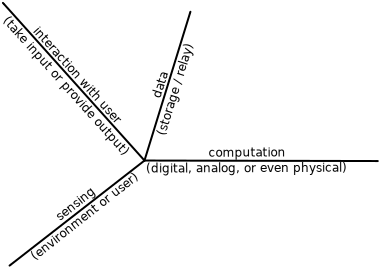
\includegraphics[width=.8\linewidth]{figures/4axes.png}
		\includegraphics[width=1\linewidth]{figures/amazon wearable technology.png}
	\end{frame}
	
\end{document}
